% Section 1.1: Evidence for Dark Matter

\section{Evidence for Dark Matter}
\label{sec:1.1}
% The case for dark matter rests on a convergence of independent lines of evidence spanning a wide range of astrophysical scales.
Evidence of the existance of dark matter spans a wide range of astrophysical scales.
We follow the hierarchical classification of Cirelli et al.~\cite{Cirelli:2024ssz}, organizing the evidence from galactic (``mini'') to cluster (``midi'') to cosmological (``maxi'') scales.
The internal consistency of these measurements --- obtained with fundamentally different techniques, probing different physical environments --- is one of the strongest arguments in favor of a dark matter interpretation in terms of new physics. 

\subsection{Galactic Scale}
\label{sec:1.1.1}

Among the earliest and most compelling evidence for dark matter is the kinematics of galaxies.
In a spiral galaxy, the circular velocity $v_c(r)$ of stars and gas at distance $r$ from the center is determined by the enclosed mass through $v_c(r) = \sqrt{GM(r)/r}$.
If the visible mass --- concentrated in a central bulge --- was the main source of the gravitational potential, the rotation curve should decline as $v_c \propto r^{-1/2}$ beyond the luminous extent of the bulge, following the standard Keplerian falloff.

Observations tell a different story.
The first hints of anomalous galactic dynamics appeared with Babcock's 1939 study of M31, though the measurements lacked the radial extent and precision to be conclusive~\cite{Babcock:1939}.
The modern picture took shape in 1970, when Rubin and Ford~\cite{Rubin:1970zza} obtained the first high-precision optical rotation curve of M31, tracing approximately 70 H\,\textsc{ii} regions out to ${\sim}\,22$~kpc and finding no evidence of the expected Keplerian decline.
In the same year, Freeman identified similar discrepancies in the disk dynamics of several spiral galaxies~\cite{Freeman:1970}.
Over the following decades, radio observations of the 21-cm hydrogen line extended rotation curves well beyond the optical disk, establishing that $v_c(r)$ remains approximately constant out to the largest measurable radii in hundreds of systems~\cite{Rubin:1980zd,Bosma:1981zz}.
To maintain a constant circular velocity, the enclosed mass must grow linearly with radius, $M(r) \propto r$, which suggests an extended, roughly spherical halo of invisible matter with density $\rho(r) \propto r^{-2}$ at large radii.
The comprehensive analysis of Persic, Salucci, and Stel~\cite{Persic:1995ru} synthesized rotation curves across a wide range of galaxy luminosities into a ``Universal Rotation Curve'', demonstrating that the dark-to-luminous mass ratio increases systematically with decreasing galaxy luminosity.

Modern data have only strengthened this picture.
The Spitzer Photometry and Accurate Rotation Curves (SPARC) compilation~\cite{Lelli:2016zqa} provides high-quality mass models for 175 disk galaxies spanning a broad range of surface brightnesses and morphologies.
These data confirm the ubiquity of flat rotation curves and reveal tight empirical scaling relations --- such as the baryonic Tully-Fisher relation linking asymptotic rotation velocity to total baryonic mass~\cite{Trully1977, McGaugh:2000sr} --- that any successful dark matter model must reproduce.
Figure~\ref{fig:rotation_curves} illustrates this evidence: the left panel shows the original optical rotation curve of M31 from Rubin and Ford~\cite{Rubin:1970zza}, while the right panel presents a modern mass decomposition demonstrating the dominant contribution of the dark matter halo at large radii.

%
% 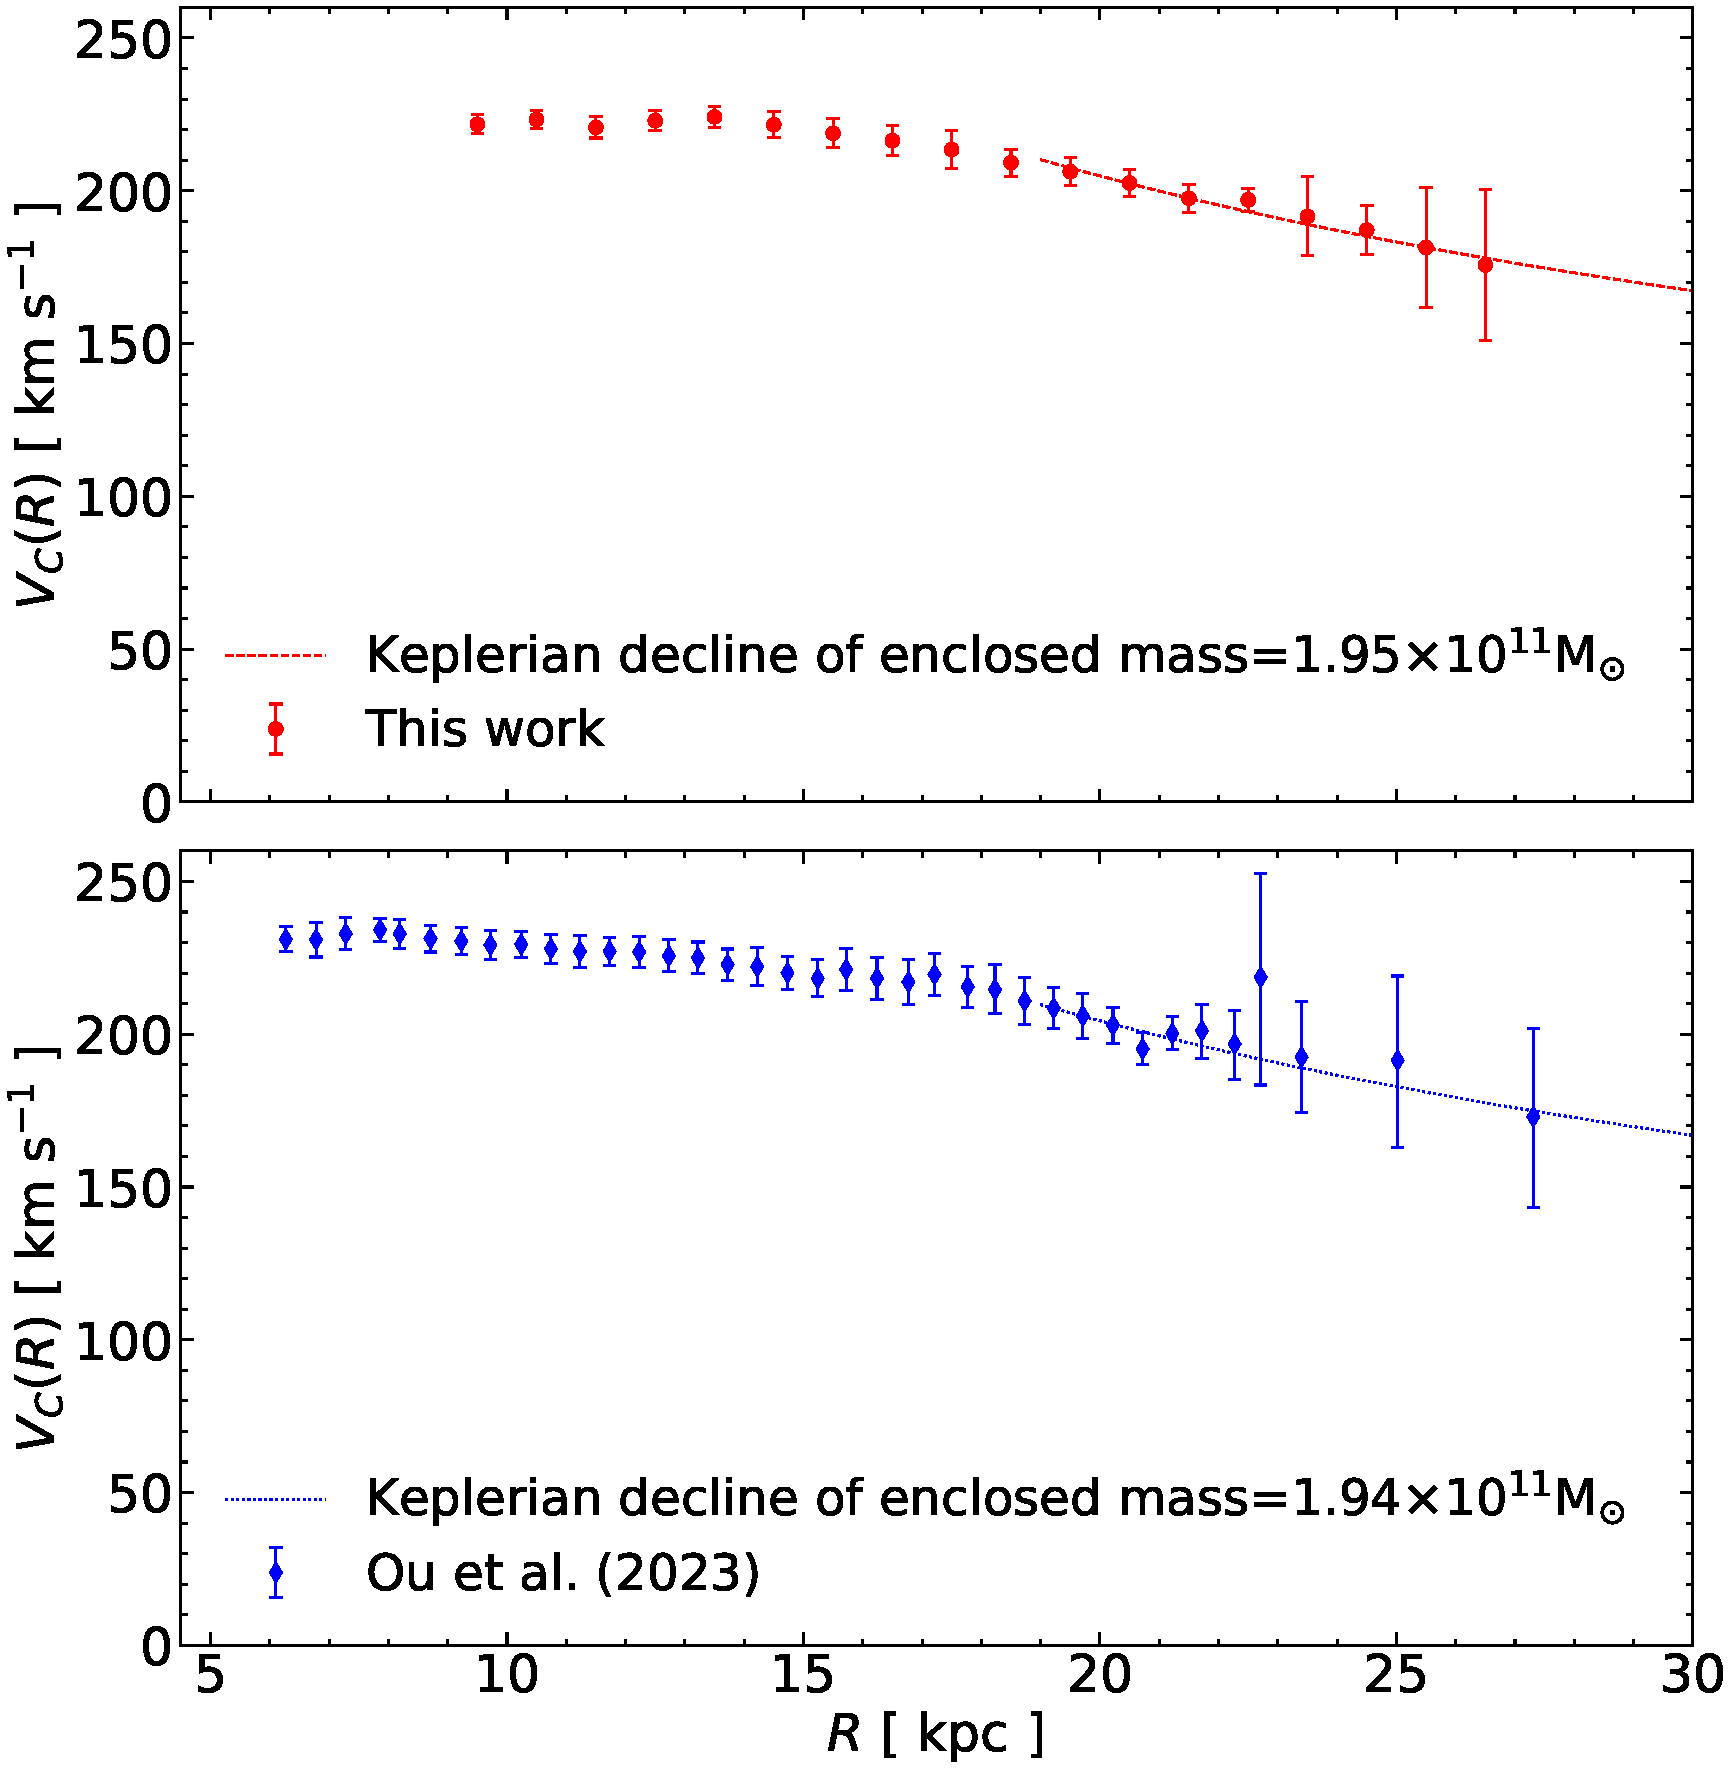
\includegraphics[width=0.45\textwidth,height=0.22\textheight]{figures/RotationCurveMW.pdf} \\[2mm]
% 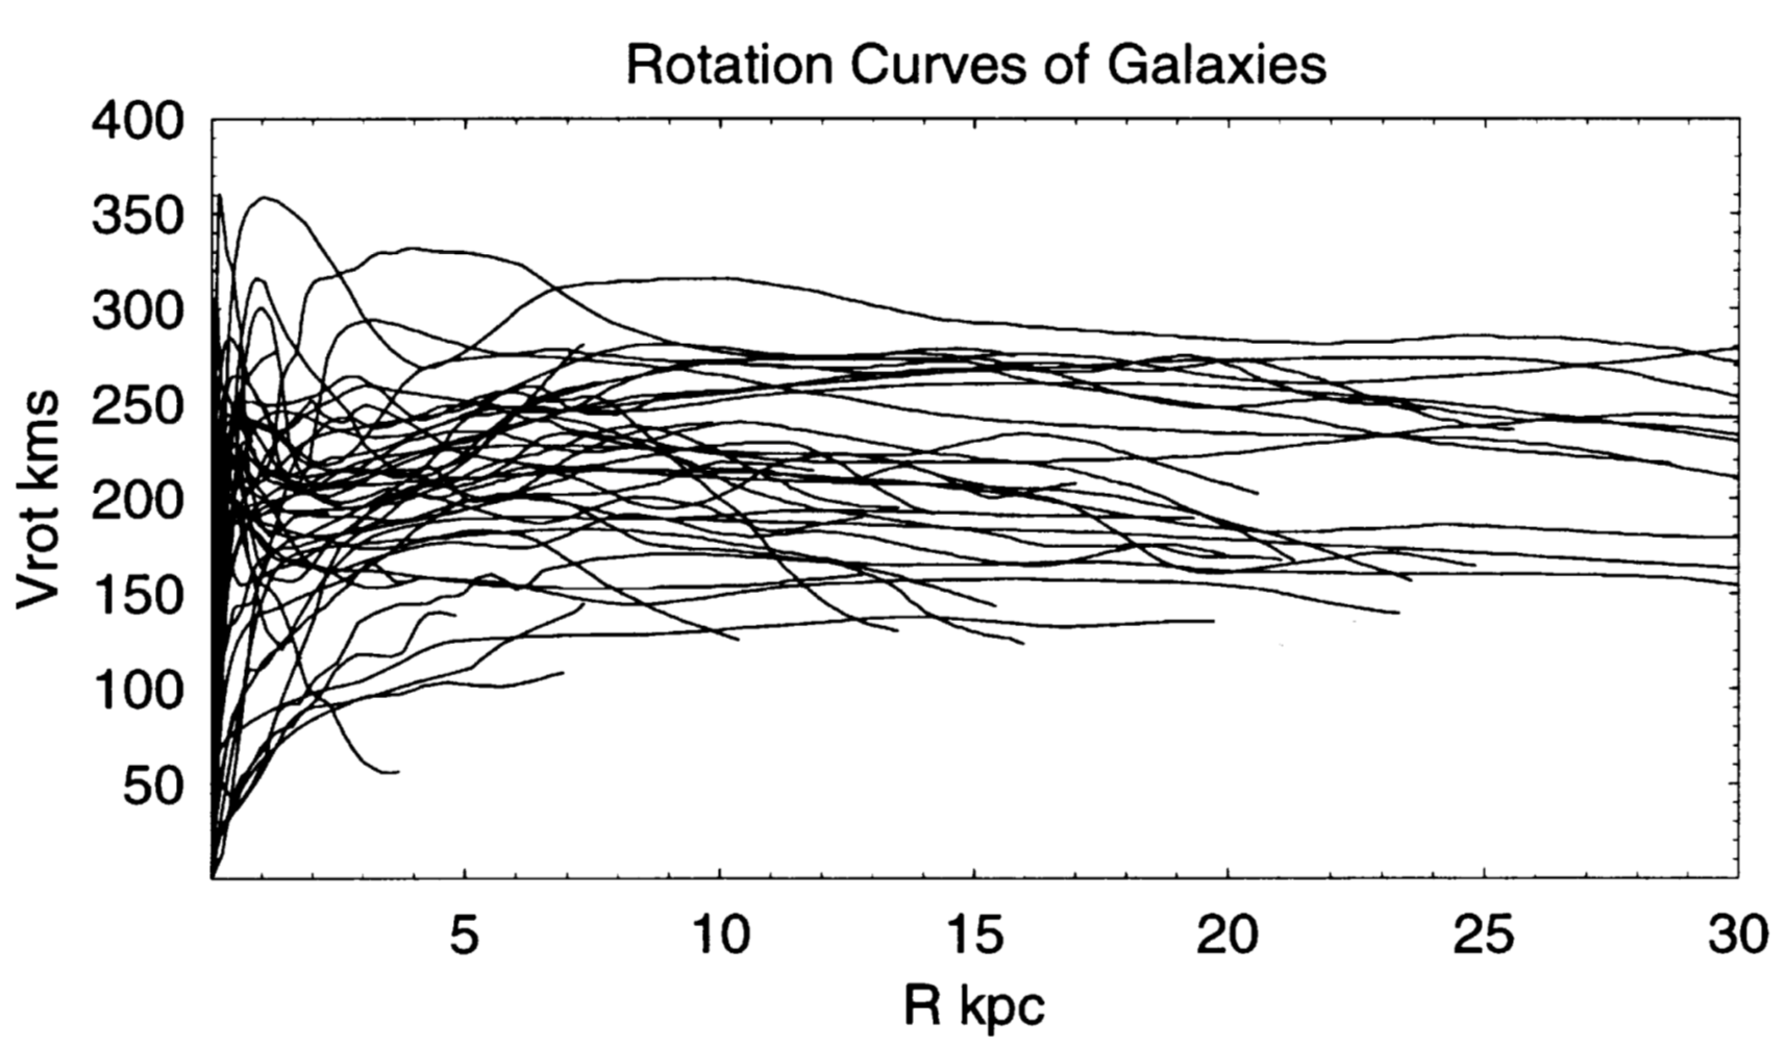
\includegraphics[width=0.45\textwidth,height=0.23\textheight]{figures/rotationcurve3_compilation_fromSofue1999.pdf}$\qquad$%
% 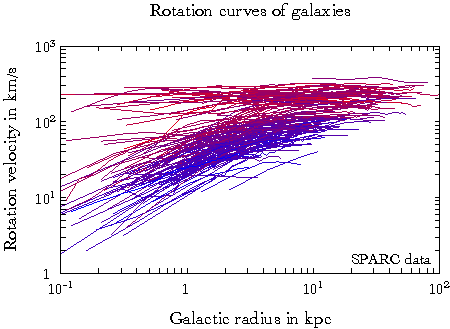
\includegraphics[width=0.44\textwidth]{figures/RotationCurveCompilationSPARC.pdf}\\[2mm]
% 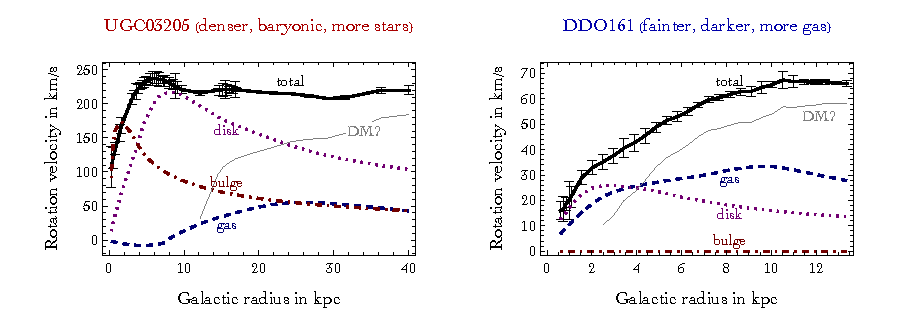
\includegraphics[width=0.97\textwidth]{figures/RotationCurveSample.pdf}
\begin{figure}[t]
	\centering
	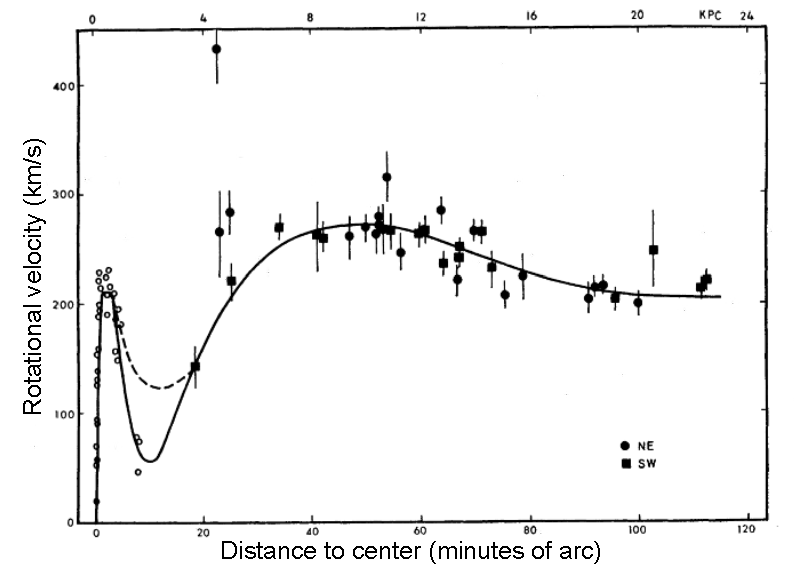
\includegraphics[width=0.45\textwidth,height=0.22\textheight]{figures/rubin-m31-v2.pdf}%
	\qquad%
	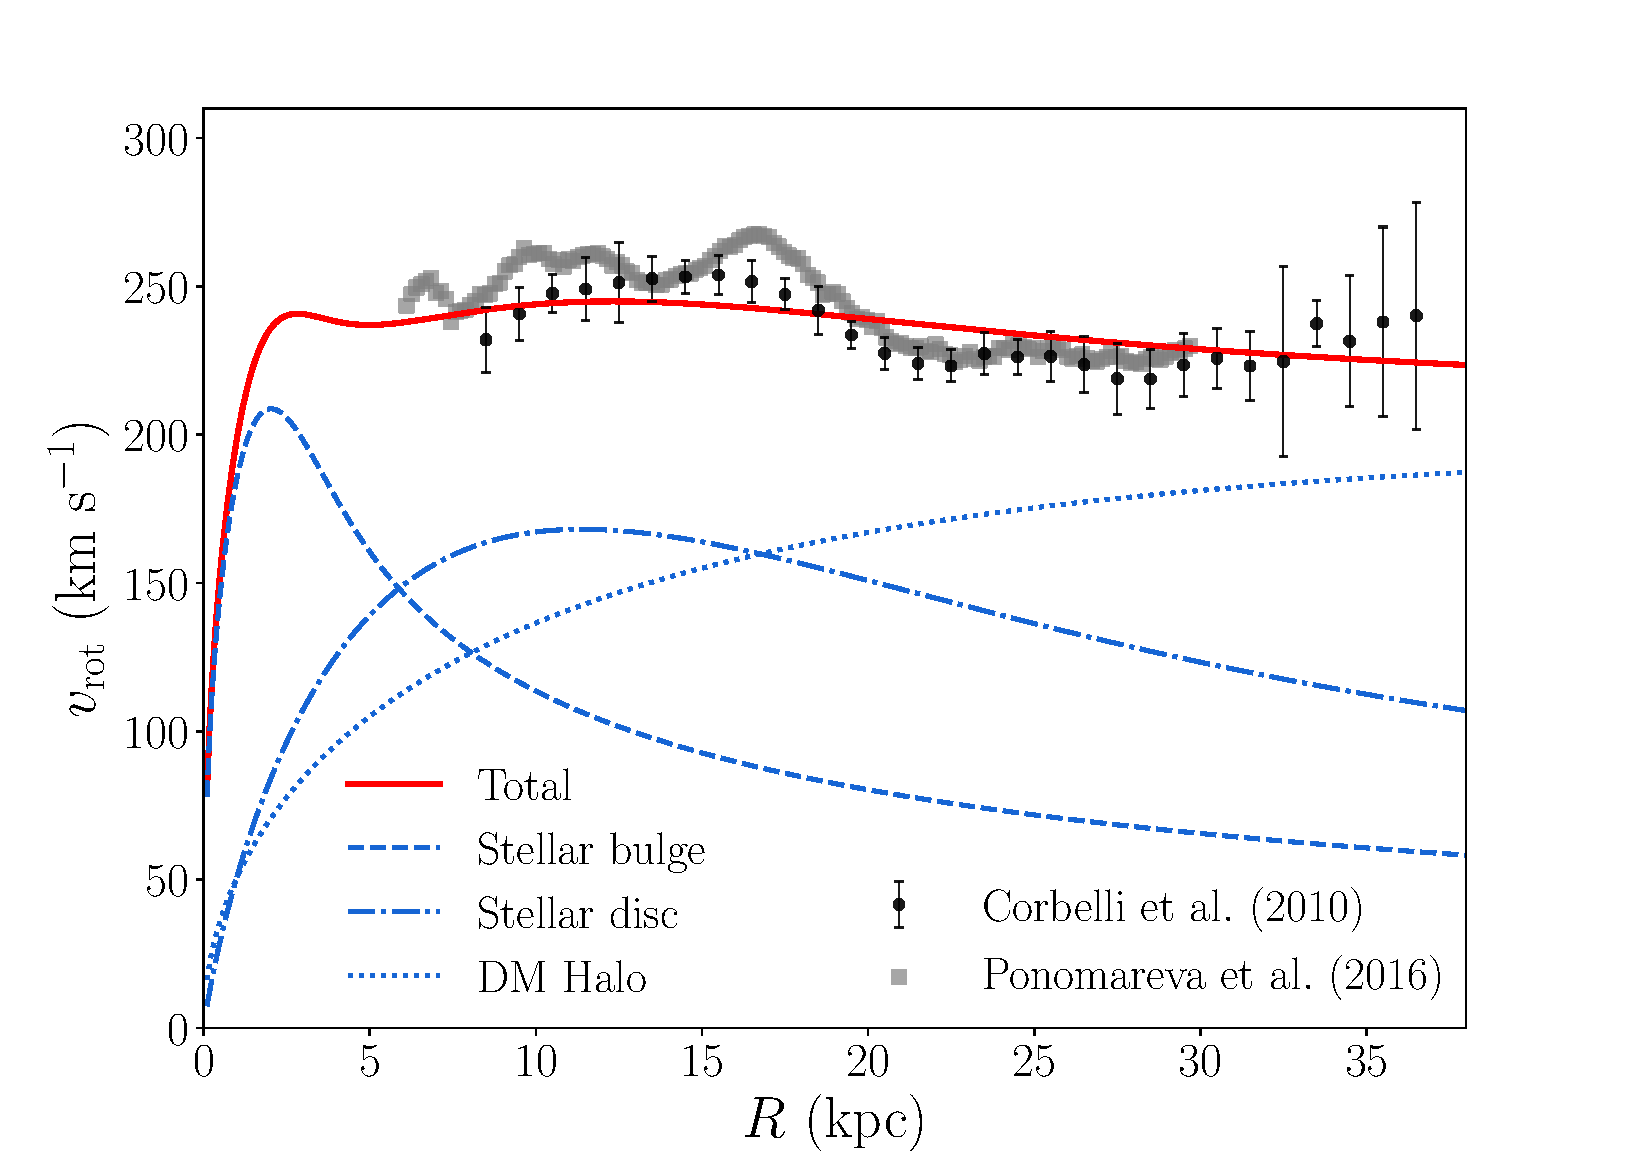
\includegraphics[width=0.45\textwidth,height=0.22\textheight]{figures/afruni-m31-decomposition.pdf}
	\caption{Rotation curves and mass decomposition of M31.
		\textit{Left}: the original optical rotation curve measured by Rubin and Ford~\cite{Rubin:1970zza}, one of the first datasets to show that the observed velocities do not follow the expected Keplerian decline.
		\textit{Right}: a modern mass decomposition from Afruni et al.~\cite{Afruni:2021}, showing the contributions of the stellar disk, gas, and dark matter halo to the total rotation curve; the dark matter halo dominates at large radii.
	}
	\label{fig:rotation_curves}
\end{figure}

An independent line of evidence comes from the satellite galaxies of the Milky Way.
\Glspl{dSph_} --- small, gas-poor stellar systems such as Draco, Sculptor, and Segue~1 --- orbit within the gravitational potential of our Galaxy and represent some of the smallest and faintest galaxies known.
Unlike the disk galaxies discussed above, stars in \glspl{dSph_} move on essentially random orbits, making these systems pressure-supported rather than rotationally supported.
The simple relation $v_c(r) = \sqrt{GM(r)/r}$ that governs rotating disks is therefore not directly applicable, and the enclosed mass is instead inferred from the line-of-sight velocity dispersion $\sigma_*$ of the stellar population.
Wolf et al.~\cite{Wolf:2009tu} showed that the mass enclosed within the three-dimensional half-light radius is robustly estimated by $M(<r_{1/2}) \approx 3\sigma_*^2 r_{1/2} / G$, a result that is largely insensitive to the unknown velocity anisotropy.
Applying this estimator reveals extreme mass-to-light ratios: from $M/L \sim 10\,M_\odot/L_\odot$ in the classical dwarfs, to several hundred in Draco ($M/L \sim 300$), to well over a thousand in ultra-faint systems like Segue~1~\cite{Walker:2009zp,Wolf:2009tu}.
These ratios cannot be explained by baryonic mechanisms alone, establishing \glspl{dSph_} as the most dark-matter-dominated objects known.
Their low astrophysical backgrounds also make them prime targets for indirect dark matter searches, a point to which we return in Section~\ref{sec:targets}.

\subsection{Galaxy Cluster Scale}
\label{sec:1.1.2}

Moving to larger scales, the dynamics of galaxy clusters provide another class of evidence for dark matter.
The earliest quantitative argument dates back to 1933, when Fritz Zwicky studied the radial velocities of galaxies in the Coma Cluster~\cite{Zwicky:1933}.
Applying the virial theorem --- which relates the time-averaged kinetic energy of a gravitationally bound system to its potential energy, $2\langle K \rangle + \langle U \rangle = 0$ --- he estimated the cluster's total mass and found a mass-to-light ratio of ${\sim}\,400$, far exceeding what could be accounted for by the luminous galaxies alone.
Zwicky concluded that the cluster must contain a large amount of unseen matter, to which he referred as ``dunkle materie'' --- dark matter.

Modern X-ray observations have placed these early dynamical estimates on much firmer ground.
Galaxy clusters contain massive reservoirs of ionized gas --- the \ICM --- heated to temperatures of $10^7$--$10^8$~K as it falls into the cluster potential well.
This gas radiates thermally through bremsstrahlung emission, observed in the X-ray band~\cite{Sarazin:1986zz}.
Under the assumption of hydrostatic equilibrium, the outward gas pressure gradient balances the inward gravitational pull, so the total gravitating mass can be reconstructed from the observed gas temperature and density profiles.
These analyses consistently show that the visible galaxies plus the X-ray-emitting gas account for only ${\sim}\,15\%$ of the total cluster mass~\cite{Cirelli:2024ssz}, with the rest attributable to a dark, non-luminous component.

The \SZ effect~\cite{Sunyaev:1972} offers a complementary probe.
When \CMB photons traverse a cluster, they undergo inverse-Compton scattering off the hot \ICM electrons, gaining energy and producing a characteristic spectral distortion~\cite{Bullock:2017xww}.
The amplitude of this distortion is proportional to the integrated electron pressure along the line of sight and, unlike X-ray surface brightness, does not diminish with redshift.
Combined with independent constraints on the baryon density from \BBN and the \CMB (where $\Omega_b \approx 0.05$), \SZ measurements of the cluster baryon fraction $f_b \approx \Omega_b / \Omega_m$ yield a total matter density $\Omega_m \approx 0.3$, well above the baryonic contribution~\cite{Aghanim:2018eyx}.

Gravitational lensing provides a direct method for mapping the total mass distribution of clusters, independent of assumptions about dynamical equilibrium.
Strong lensing in the dense cluster core produces highly distorted arcs and multiple images of background galaxies, while weak lensing measures the statistical shearing of background galaxy shapes over larger angular scales~\cite{Bullock:2017xww}.
Both regimes reconstruct the total mass distribution --- visible and dark --- from the geometry of light paths alone.

A striking application of gravitational lensing is the Bullet Cluster (1E\,0657-558), analyzed by Clowe et al.~\cite{Clowe:2006eq}.
This system consists of two galaxy clusters that passed through each other roughly 150 million years ago.
X-ray observations reveal that the collisional baryonic gas from the two clusters interacted strongly, producing a bow shock and lagging behind the galaxies.
Weak-lensing mass maps, however, show that the bulk of the total mass is spatially offset from the gas, coinciding instead with the collisionless galaxies.
This spatial separation is visible in Figure~\ref{fig:bullet_cluster}: the green mass contours reconstructed through weak lensing are displaced from the X-ray-emitting gas, demonstrating that the dominant mass component is collisionless.
The observed separation matches the behavior expected of collisionless dark matter and contradicts modified gravity theories such as \MOND~\cite{Milgrom:1983ca}, in which the lensing signal should trace the baryonic gas.
Harvey et al.~\cite{Harvey:2015hha} extended this analysis to 72 colliding clusters, confirming the separation of dark matter from baryonic gas at greater than $7\sigma$ significance and setting stringent upper limits on the dark matter self-interaction cross-section.

\begin{figure}[t]
	\centering
	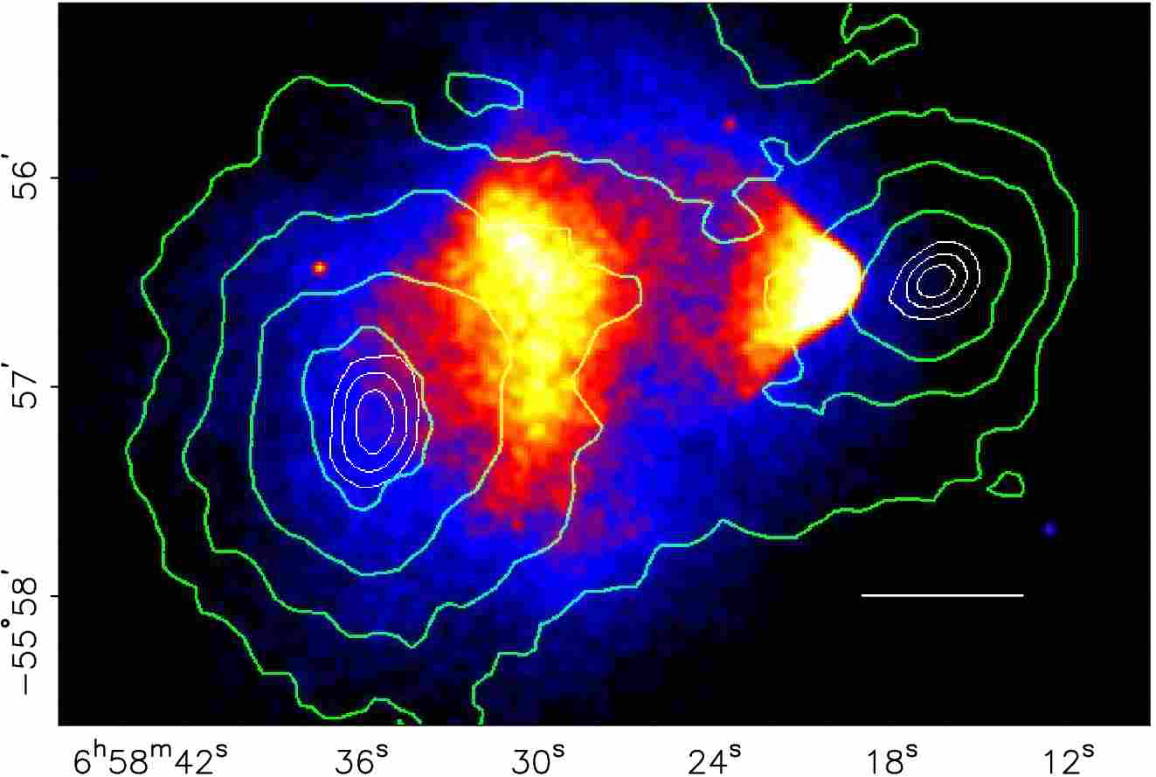
\includegraphics[width=0.6\textwidth]{figures/f1b_new_jpeg2ps.pdf}
	\caption{The Bullet Cluster (1E\,0657-558).
		The color map shows the X-ray surface brightness of the hot intracluster gas from \textit{Chandra} observations, while the green contours trace the total mass distribution reconstructed through weak gravitational lensing.
		The clear spatial offset between the two demonstrates that the dominant mass component is collisionless.
		The white bar corresponds to 200~kpc.
		Credit: Cirelli et al.~\cite{Cirelli:2024ssz}, after Clowe et al.~\cite{Clowe:2006eq}.
	}
	\label{fig:bullet_cluster}
\end{figure}

\subsection{Cosmological Scale}
\label{sec:1.1.3}

At the largest scales, precision cosmological observations provide the tightest constraints on dark matter and its non-baryonic nature.

The \CMB radiation is the thermal relic of the hot, dense early Universe.
Roughly 380,000 years after the Big Bang, the expanding cosmos cooled sufficiently for protons and electrons to combine into neutral hydrogen --- an epoch known as \emph{recombination}.
Before this transition, baryonic matter existed as a hot plasma tightly coupled to photons through Thomson scattering; after recombination, photons streamed freely, and this ``last scattering surface'' is what we observe today as the \CMB.
Its temperature is remarkably uniform at ${\sim}\,2.725$~K, but carries tiny anisotropies at the level of ${\sim}\,10^{-5}$ that encode detailed information about the matter-energy content of the cosmos.

These anisotropies are conventionally decomposed into angular scales via the temperature power spectrum $C_\ell$, which quantifies the variance of temperature fluctuations at each angular multipole $\ell$ --- with larger $\ell$ corresponding to smaller angular separations on the sky.
Peaks in $C_\ell$ correspond to sound waves in the pre-recombination baryon-photon plasma that were caught at maximum compression or rarefaction at the moment of decoupling; the positions and heights of these peaks encode the composition and geometry of the Universe~\cite{Aghanim:2018eyx,Cirelli:2024ssz}.
Baryons load the oscillating fluid, enhancing the compressional (odd-numbered) peaks relative to the rarefaction (even-numbered) ones, so that the ratio of the first to the second peak directly constrains the physical baryon density.
Dark matter, which does not couple to the photon pressure, provides the gravitational scaffolding within which the oscillations occur: its abundance sets the overall depth of the potential wells and modulates the relative heights of successive peaks.
In particular, a universe without cold dark matter would produce a strongly suppressed third peak (cf.\ Figure~\ref{fig:cmb}), in clear contradiction with the observed spectrum.
The Planck 2018 analysis yields $\Omega_c h^2 = 0.1200 \pm 0.0012$ for the cold dark matter density and $\Omega_b h^2 = 0.02237 \pm 0.00015$ for the baryon density~\cite{Aghanim:2018eyx}, suggesting that dark matter is roughly five times more abundant than ordinary matter.
Figure~\ref{fig:cmb} illustrates the contrast between the observed spectrum and the prediction for a baryon-only universe.

\begin{figure}[t]
	\centering
	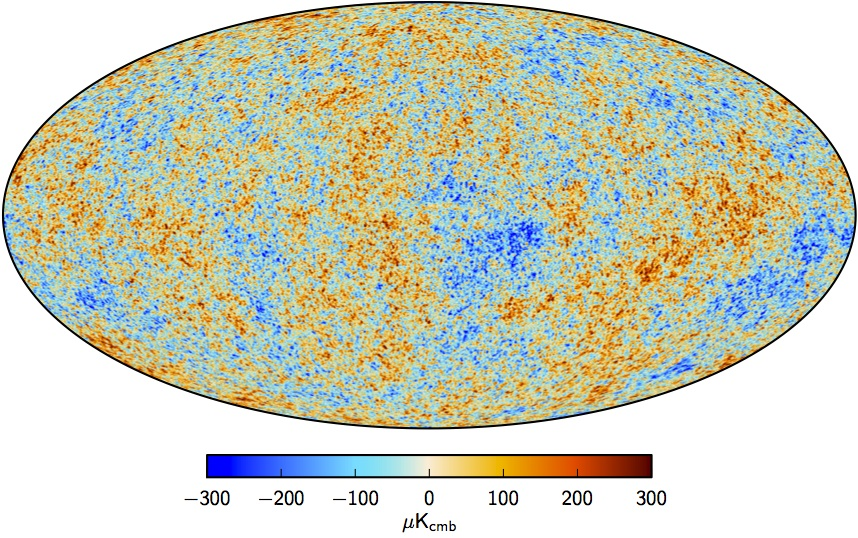
\includegraphics[width=0.65\textwidth]{figures/CMB_PlanckMap.jpg}\\[2mm]
	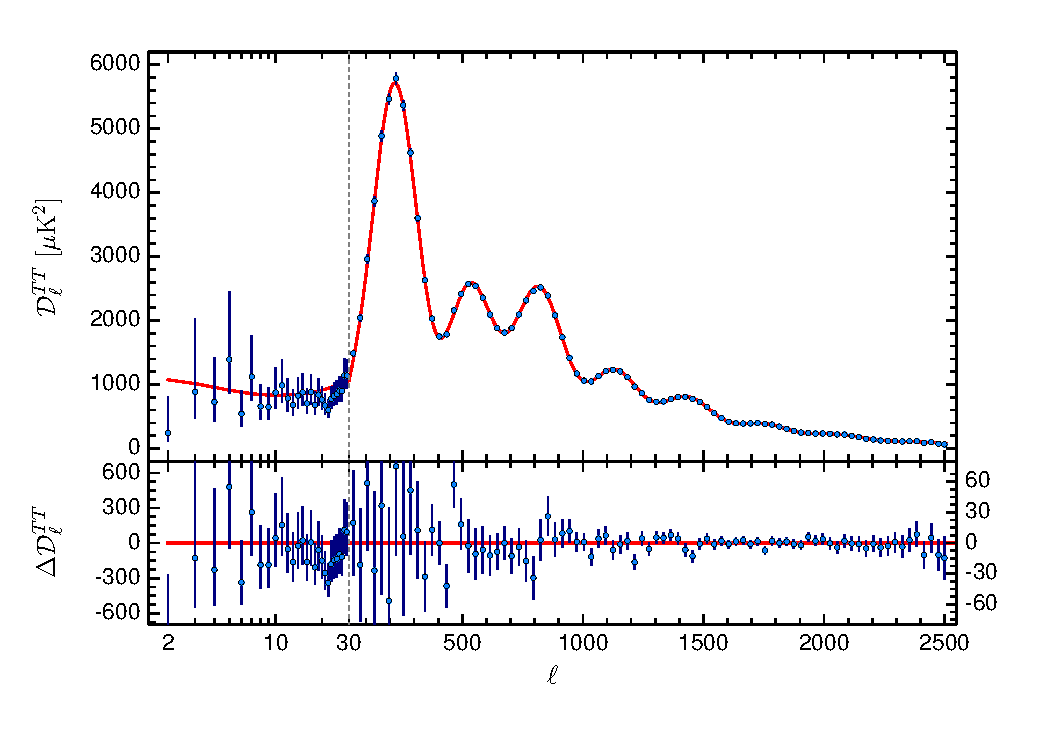
\includegraphics[width=0.47\textwidth]{figures/CMB_Planck2014_TT.pdf}~%
	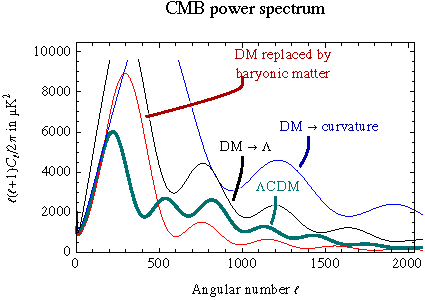
\includegraphics[width=0.47\textwidth,height=170pt]{figures/CMBnoDMAS.pdf}
	\caption{The imprint of dark matter on the \CMB.
		\textit{Top}: the Planck \CMB temperature anisotropy map~\cite{Aghanim:2018eyx}, showing the ${\sim}\,10^{-5}$ fluctuations in the otherwise uniform 2.725~K radiation field.
		\textit{Bottom left}: the observed angular power spectrum $C_\ell^{TT}$ of the \CMB temperature anisotropies, measured by the Planck satellite~\cite{Aghanim:2018eyx}.
		% \textit{Bottom right}: the same quantity computed in a universe without cold dark matter, showing the dramatic suppression of the third acoustic peak.
		\textit{Bottom right}: the same quantity computed in several different cosmological scenarios. The green line represents the best-fit $\Lambda$CDM model, while the red line shows the prediction for a universe without cold dark matter, which fails to reproduce the observed third acoustic peak.
		Adapted from the Planck Collaboration~\cite{Aghanim:2018eyx} and Cirelli et al.~\cite{Cirelli:2024ssz}.
	}
	\label{fig:cmb}
\end{figure}

\begin{figure}[t]
	\centering
	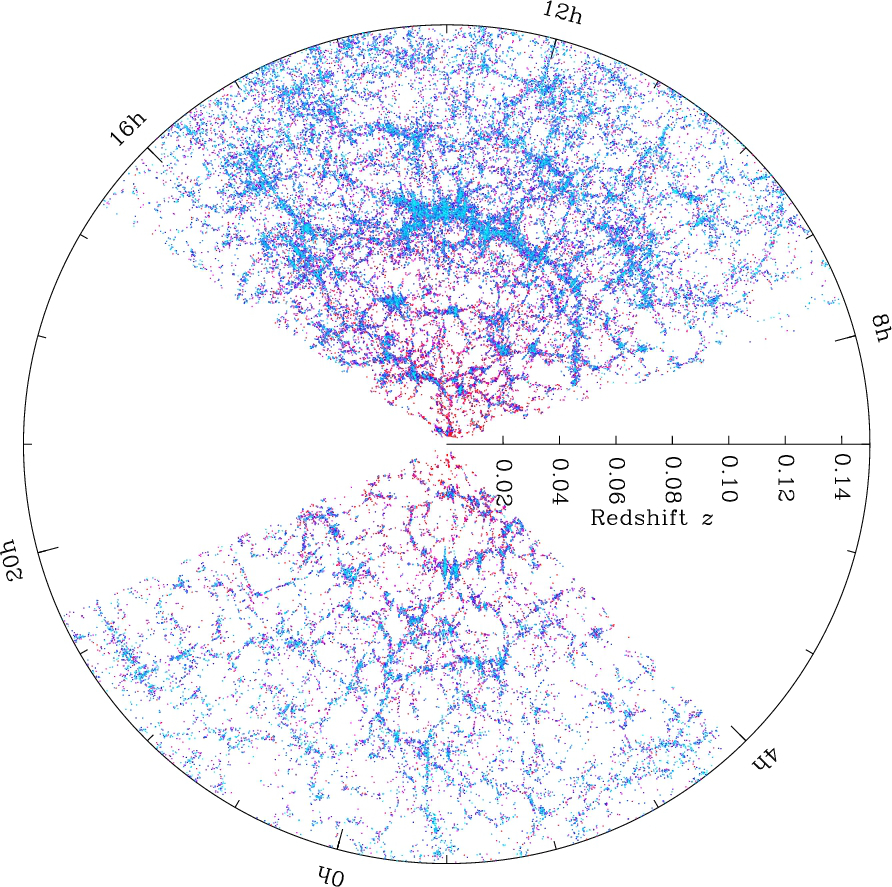
\includegraphics[width=0.50\textwidth]{figures/LSS_sdss_release14-inverted.jpg}\\[2mm]
	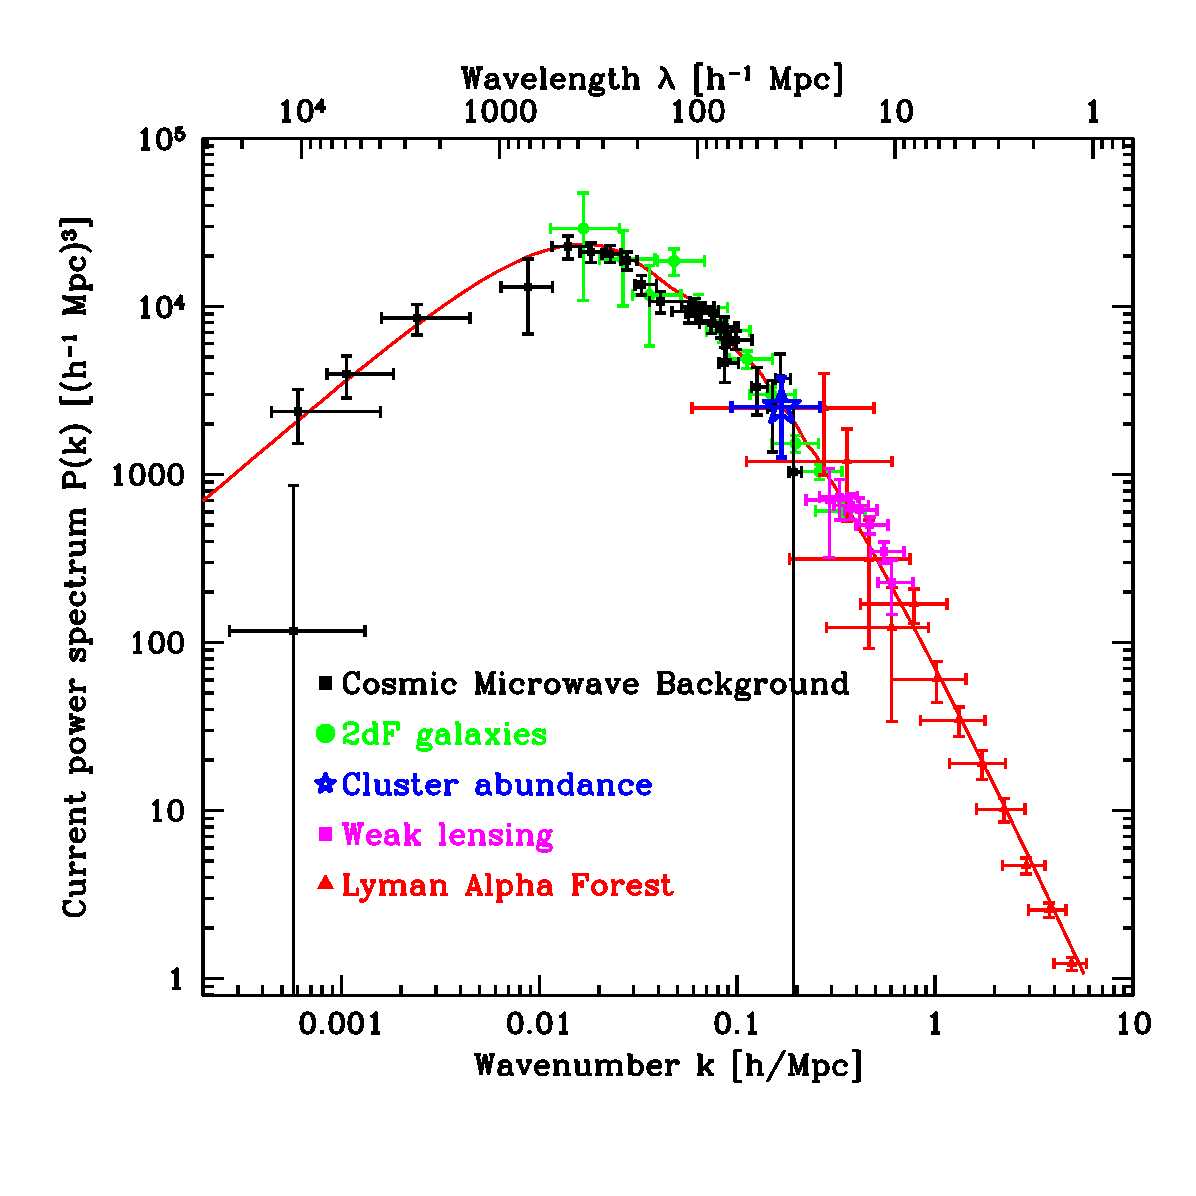
\includegraphics[width=0.47\textwidth,height=170pt]{figures/LSS_powerspectrum.pdf}~%
	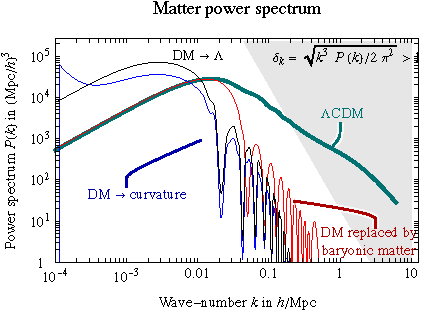
\includegraphics[width=0.47\textwidth]{figures/LSSpowerDMAS.pdf}
	\caption{The imprint of dark matter on large-scale structure.
		\textit{Top}: the large-scale distribution of galaxies from the Sloan Digital Sky Survey (SDSS)~\cite{eBOSS:2017pfi}.
		\textit{Bottom left}: the observed matter power spectrum $P(k)$~\cite{Tegmark:2002cy}.
		\textit{Bottom right}: the same quantity computed in several different cosmological scenarios. The green line represents the best-fit $\Lambda$CDM model, while the red line shows the prediction for a universe without cold dark matter, in which power on small (large-$k$) scales is strongly suppressed --- reflecting the absence of small-scale structure~\cite{Dodelson:2006zt}.
		Adapted from the SDSS Collaboration~\cite{eBOSS:2017pfi}, Tegmark and Zaldarriaga~\cite{Tegmark:2002cy}, and Cirelli et al.~\cite{Cirelli:2024ssz}.
	}
	\label{fig:lss}
\end{figure}

The observed large-scale structure of the Universe delivers a complementary argument for dark matter.
In a purely baryonic universe, structure formation would have been severely hindered: before recombination, baryons were tightly coupled to photons through Thomson scattering, and their density perturbations were erased on small scales by photon diffusion --- a process known as \emph{Silk damping}~\cite{Silk:1967kq}.
Cold dark matter, which does not interact electromagnetically, is immune to this damping and began to cluster gravitationally during the matter-dominated era, well before recombination~\cite{Davis:1985rj}.
The potential wells established by dark matter then acted as seeds into which baryons fell after decoupling, seeding the formation of galaxies and clusters (see Section~\ref{sec:5.2} for a more detailed treatment of dark matter halo formation and substructure).
Without this pre-existing dark matter framework, the matter power spectrum $P(k)$ cannot be reproduced; Figure~\ref{fig:lss} illustrates the striking difference in predicted large-scale structure between a universe with and without cold dark matter.

Beyond the overall shape of the matter power spectrum, the primordial sound waves left a second, sharper imprint on the distribution of matter.
\Gls{BAO_} preserve this imprint in the large-scale galaxy distribution.
The same pressure waves that produced the acoustic peaks in the \CMB power spectrum were also imprinted on the baryonic matter: when the baryon-photon plasma decoupled at recombination, the outward-propagating sound shells froze in place, leaving a characteristic comoving scale of ${\sim}\,150$~Mpc in the spatial correlations of galaxies.
This scale appears as a well-defined bump in the two-point correlation function and provides a ``standard ruler'' for measuring the expansion history of the Universe.
Its first detection in the galaxy distribution by Eisenstein et al.~\cite{SDSS:2005xqv} delivered independent confirmation of the $\Lambda$CDM parameters.
\BAO measurements of the expansion rate, combined with distance measurements from Type~Ia supernovae --- which established the accelerated expansion of the Universe~\cite{SupernovaSearchTeam:1998fmf,SupernovaCosmologyProject:1998vns} --- and \CMB data, constrain the dark energy density to $\Omega_\Lambda \approx 0.7$ and the total matter density to $\Omega_m \approx 0.3$~\cite{Aghanim:2018eyx,Pan-STARRS1:2017jku}.

So far we have pointed out that the total matter density is $\Omega_m h^2 \approx 0.14$, while the \CMB independently constrains the baryon density to $\Omega_b h^2 \approx 0.022$~\cite{Aghanim:2018eyx} --- so the dark, supposedly non-baryonic component outweighs ordinary matter by roughly a factor of five.
Could this missing matter simply be a form of ordinary matter that happens to be dark: cold molecular gas clouds, compact stellar remnants, or some as-yet-undetected baryonic component hiding in the intergalactic medium?
\BBN decisively rules out this possibility.
The production of light elements during the first few minutes after the Big Bang is highly sensitive to the baryon-to-photon ratio, and the observed primordial abundances of deuterium, $^4$He, and $^7$Li independently constrain the baryon density to $\Omega_b h^2 \approx 0.022$~\cite{Iocco:2008va,ParticleDataGroup:2022pth} --- in agreement with the \CMB, but through entirely different physics.
Crucially, this constraint applies to the \emph{total} baryon density, not just the visible fraction: any baryonic matter, however dark or diffuse, would have participated in nucleosynthesis and altered the primordial element yields
% The observed abundances leave no room for a hidden baryonic reservoir.
Whatever dark matter is, it must therefore be predominantly \emph{non-baryonic}\footnote{The one notable exception is \emph{primordial black holes}, which form from the gravitational collapse of large density perturbations before nucleosynthesis: having decoupled from the baryon budget so early, they behave as effectively non-baryonic dark matter, even though they invoke no new particle species (cf.\ Section~\ref{sec:1.2.1}). In the remainder of this thesis, whenever we state that dark matter cannot be composed of Standard Model particles, this exception is left implicit.} --- a new form of matter beyond the Standard Model.

In the next section we introduce and explore the \WIMP paradigm, one of the most popular and well-motivated particle physics candidate for dark matter.

% --- a conclusion that motivates the particle physics discussion of the following section.
